\documentclass[../report.tex]{subfiles}
\begin{document}
    
    \begin{frame}
        \frametitle{4a: PF Occlusions}
        \begin{figure}[!htb]
            \centering
            \frame{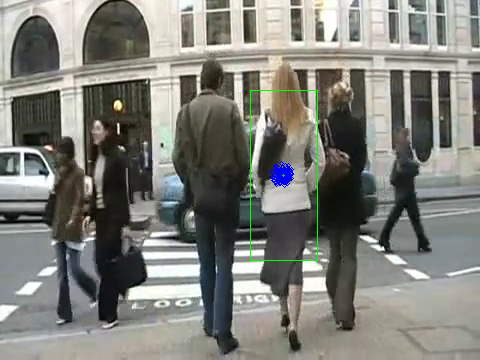
\includegraphics[keepaspectratio,height=0.65\textheight,width=0.45\textwidth]{ps5-4-a-1}}
            \caption{ps5-4-a-1}
        \end{figure}
    \end{frame}

    \begin{frame}
        \frametitle{4a: PF Occlusions (cont.)}
        \begin{figure}[!htb]
            \centering
            \frame{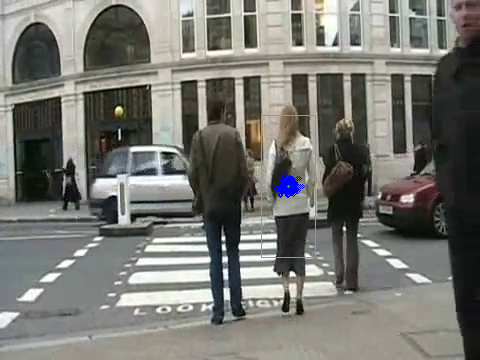
\includegraphics[keepaspectratio,height=0.65\textheight,width=0.45\textwidth]{ps5-4-a-2}}
            \caption{ps5-4-a-2}
        \end{figure}
    \end{frame}

    \begin{frame}
        \frametitle{4a: PF Occlusions (cont.)}
        \begin{figure}[!htb]
            \centering
            \frame{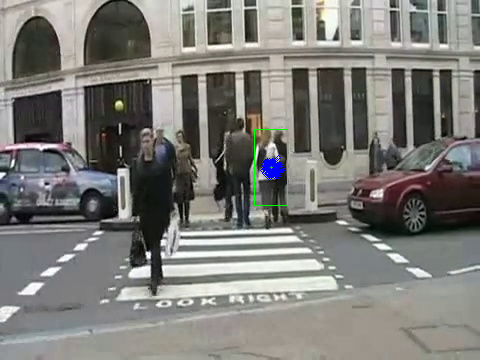
\includegraphics[keepaspectratio,height=0.65\textheight,width=0.45\textwidth]{ps5-4-a-3}}
            \caption{ps5-4-a-3}
        \end{figure}
    \end{frame}

    \begin{frame}
        \frametitle{4a: PF Occlusions (cont.)}
        \begin{figure}[!htb]
            \centering
            \frame{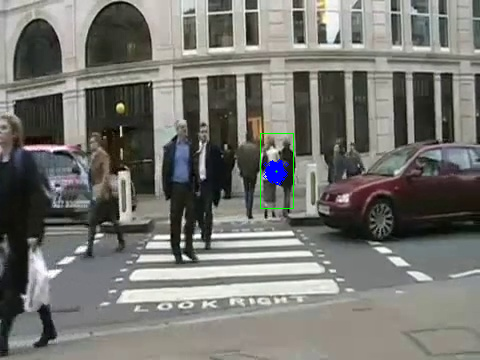
\includegraphics[keepaspectratio,height=0.65\textheight,width=0.45\textwidth]{ps5-4-a-4}}
            \caption{ps5-4-a-4}
        \end{figure}
    \end{frame}

    \begin{frame}[t]
        \frametitle{4: Text response}
        \begin{normalsize}
            \begin{itemize}
                \setlength\itemsep{1em}\fontsize{6pt}{6pt}

                \item[]{\textbf{\selectfont\textcolor{blue}{ Describe what you did. How did you modify the Particle Filter class to continue tracking after occlusions? }}}
                
                \item[]\textbf{\documentclass[../report.tex]{subfiles}
\begin{document}
    \begin{frame}
    	\frametitle{Multiple Sign Detection With Noise}
    	\begin{table}[!htb]
        \centering
        \begin{tabular}{ c m{5cm} }
        
            \begin{minipage}{.45\textwidth}
            \frame{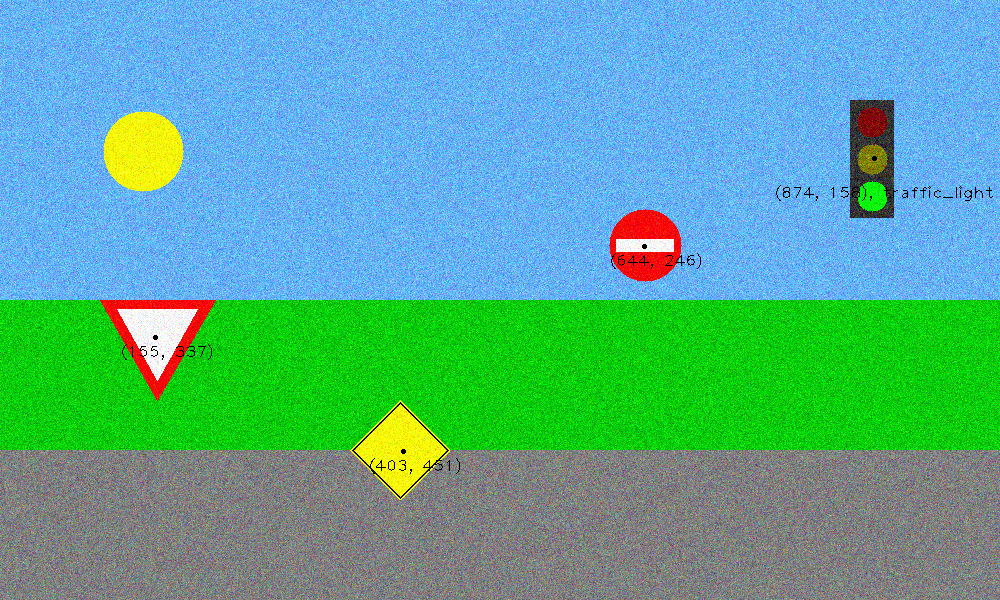
\includegraphics[keepaspectratio,height=0.7\textheight,width=1\textwidth]{ps2-4-a-1}}
                \captionof{figure}{ps2-4-a-1}
            \end{minipage}
            &
            \begin{minipage}{.45\textwidth}
                Coordinates and Name: \\
                No Entry: (-1, -1) \\
No Entry: (-1, -1) \\
No Entry: (-1, -1) \\
No Entry: (-1, -1) \\
            \end{minipage}
        
        \end{tabular}
        \end{table}
    \end{frame}
    
    \begin{frame}
    	\frametitle{Multiple Sign Detection With Noise}
    	\begin{table}[!htb]
        \centering
        \begin{tabular}{ c m{5cm} }
        
            \begin{minipage}{.45\textwidth}
            \frame{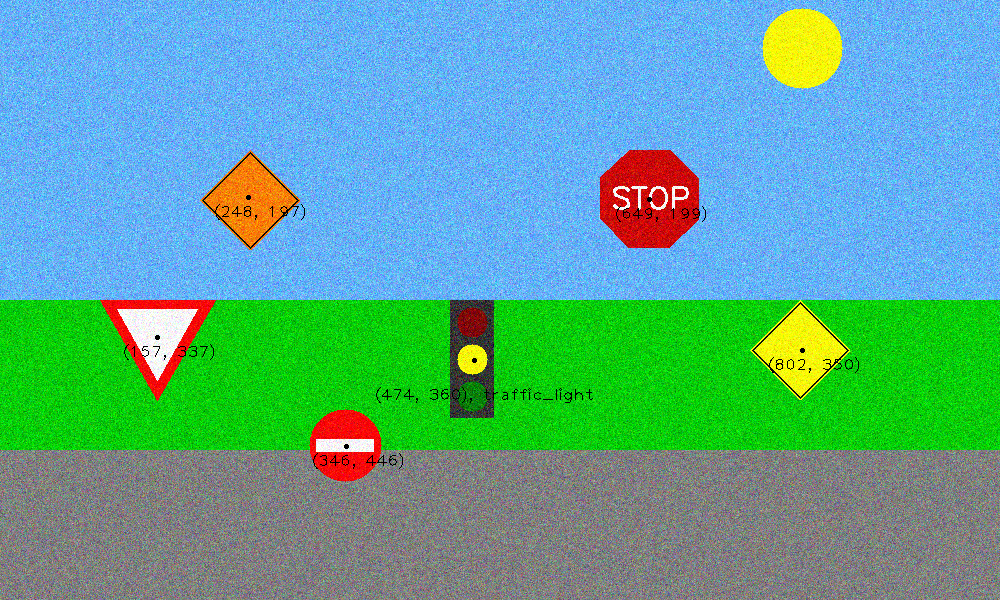
\includegraphics[keepaspectratio,height=0.7\textheight,width=1\textwidth]{ps2-4-a-2}}
                \captionof{figure}{ps2-4-a-2}
            \end{minipage}
            &
            \begin{minipage}{.45\textwidth}
                Coordinates and Name: \\
                No Entry: (-1, -1) \\
No Entry: (-1, -1) \\
No Entry: (-1, -1) \\
No Entry: (-1, -1) \\
No Entry: (-1, -1) \\
No Entry: (-1, -1)
            \end{minipage}
        
        \end{tabular}
        \end{table}
    \end{frame}
    
\end{document}}
            \end{itemize}
        \end{normalsize}
    \end{frame}

    
\end{document}